Chapter 1

\section{Abstract}

, with specific application to ray-\\finned fishes (Chordata: Actinopterygii)

A case study on ray-finned fishes retrieved from the Barcode of Life Data Systems \cite{ratnasingham2007bold} clearly highlights this shortcoming, along with the need to develop approaches which incorporate more species-level \\ information. 

A case study on DNA \\ barcoding of ray-finned fishes is then used to illustrate the need for new methods that incorporate more genomic information. Finally, qualities that a new method should possess are proposed. 

Chapter 2

\section{Haplotype Networks}

, such as the one shown in \textbf{Figure 2.1}, 

\begin{figure}[H]

\centering

\includegraphics[width=0.5\textwidth]{"Network".png}

\caption[Labelled haplotype network showing a skewed distribution of haplotypes for Longfin damselfish (\textit{Stegastes diencaeus}).]{Longfin damselfish (\textit{Stegastes diencaeus}) TCS \cite{templeton1992cladistic} haplotype network depicting an overall skewed distribution of observed haplotypes. Sizes of circles reflect the number of DNA sequences contained within each vertex. Tick marks indicate the number of mutational differences separating sampled haplotypes. DNA barcode sequence data used in the generation of the network were taken from supplemental material accompanying Phillips \textit{et al.} \cite{phillips2015exploration}. The software PopArt \cite{leigh2015popart} was used to create the haplotype network.}

\end{figure}

\section{Past Studies}}

a mathematically equivalent approach to Holt \textit{et al.}'s \cite{holt2007experimental} study through utilizing


\subsection{DNA Barcoding}

Since its inception in 2003, DNA barcoding \cite{hebert2003biological} has risen to become the largest \\ taxonomically-driven biodiversity initiative to date aimed at identifying and cataloging all assemblages of multicellular life on the planet. DNA barcoding is a genomic technique that relies on DNA sequence variation within short, standardized gene regions to rapidly identify specimens to the level of species and to discover new species. The ideal DNA barcode is one that is found in all organisms, readily distinguishes between taxa, and is easily amplified, sequenced and aligned. In animals, the agreed-upon marker of choice for taxon assignment is a \textit{c.} 650 basepair (bp) fragment from the 5' end of the \\ mitochondrially-encoded cytochrome \textit{c} oxidase subunit I (COI) gene. Mitochondrial loci like COI are particularly suitable as genetic markers for DNA barcoding because they are fast evolving, highly conserved across taxa, present in high copy number, haploid, maternally inherited, lack introns, display few insertion-deletion (indel) mutations, and experience little to no gene recombination \cite{hebert2003biological, hebert2003barcoding}.



The primary goal of DNA barcoding has been to develop a publicly accessible species reference sequence library to aid in the identification of unknown specimens and accelerate the discovery of potentially undescribed taxa. Obtaining adequate sample sizes for building accurate and reliable specimen reference libraries has culminated in the development of the Barcode of Life Data Systems (BOLD; http://www.boldsystems.org) \cite{ratnasingham2007bold} as the largest collection of user-curated species sequence data specifically for DNA barcoding currently available on the World Wide Web. At present (as of May 1, 2018), BOLD holds over six million DNA barcode records from over 250,000 named species. Certain taxa are well represented in BOLD with upwards of hundreds of barcode sequences for some species. Despite this, barcode reference libraries within BOLD remain largely incomplete, even for the most well-sampled taxa such as fishes and insects. As such, comprehensive coverage of species genetic diversity is still decades away \cite{wilkinson2017replacing}. Wilkinson \textit{et al.} \cite{wilkinson2017replacing} points to strong ascertainment bias as the most likely explanation for this. In the early days of BOLD, DNA barcode sequence acquisition was high, due to the fact that over 75\% of taxon records were mined from already well-established sequence databases such as GenBank \cite{wilkinson2017replacing}.

\subsection{Consideration of Species' Life Histories}

Life history traits, particularly those pertaining to reproductive strategies and sex \\ determination, in well-studied metazoan taxa such as fishes, insects and herpetofauna, are presumed to play a significant role in observed patterns of mtDNA barcode sequence variation at the species level. For instance, the high occurrence of haplodiploidy, a mode of inheritance whereby females develop from fertilized eggs (hence are diploid), while males arise from unfertilized eggs (therefore are haploid), is common across many insect orders such as Hymenoptera, and may explain the large abundances and varying (effective) population sizes seen in representative species that ultimately drives speciation and \\ hybridization \cite{hebert2016counting}. Similar ``exceptions to the rule", such as (asexual) modes of \\ parthenogenesis (\textit{e.g.}, unfertilized eggs producing female-only offspring in Squamata such as species of whiptail lizards), or paternal/biparental organelle inheritance in bivalve \\ molluscs (\textit{e.g.}, mussels of the genus \textit{Mytilus}), will likely help inform researchers on the required level of sampling depth needed to fully characterize broad ranges of COI haplotype diversity in taxa that do not otherwise conform to traditional mtDNA inheritance patterning (\textit{i.e.}, strictly maternal lineage), and thus prevent the na\"ive implementation of \\ recommendations of any one statistical approach employed in the calculation of \\ intraspecific sample sizes for accurate specimen assignment and rapid species delineation. As an example, because parthenogenetic species display lower standing genetic diversity compared to fully sexually-reproducing species (as a result of being exact clones of their parent due to lack of chromosomal recombination) \cite{bengtsson2003genetic}, haplotype frequencies aside, the observation of the faster approach of haplotype accumulation curves to an asymptote is expected. Thus, species exhibiting such mechanisms will require reduced levels of \\ sampling effort. Such a result can be invoked through consideration of Muller's ratchet, as the irreparable accumulation of deleterious mutations that are fixed by genetic drift within asexual genomes directly limits the ability of a species to survive and reproduce \cite{felenstein1974evolutionary, muller1964relation}. 


\section{Case Study: Phillips \textit{et al.} (2015)}

Phillips \textit{et al.} \cite{phillips2015exploration} wished to estimate \textit{sampling sufficiency} ($\theta$) \textemdash \hspace{1mm} the sample size at which accuracy is maximized and above which no additional sampling information is likely to be gained. This was applied in the context of haplotype accumulation curves to determine the point on the \textit{x}-axis where curve saturation first becomes evident. If such an estimate exists, it would provide a useful stopping rule for specimen sampling \cite{phillips2015exploration}. That is, if a lower bound for specimen sample size exists, then it would provide the best estimate of sampling sufficiency for a given species.

 Such findings may be due to the underlying assumptions of the model, which are likely to be over-simplistic, particularly that of equality of intraspecific haplotype frequencies. Further, the proposed estimator for the calculation of total haplotype diversity (\textit{H}*) (Equation 6) may be a gross overestimate. Despite not being realistic for populations of real species, the reason for adopting a uniform distribution of haplotypes was due to mathematical convenience, to make calculations of sample size as simple and as straightforward as possible. This is commonly done in practice, since determining the true distribution of species haplotypes is likely strongly dependent on species under study. Thus, values of \textit{N}* are likely overestimates of the true number of specimens that must be randomly sampled to observe most haplotype variation that exists for a species \cite{phillips2015exploration}. Phillips \textit{et al.} \cite{phillips2015exploration} argue that the use of a limited number of points in the calculation of curve slopes may not be adequate; the authors argue that a fixed proportion of curve points should instead be used. Further, through successively targeting the last 20-15\%, 15-10\% and the last 10\% of species haplotype accumulation curves, to observe a statistically-significant change in slope values, the precise point of saturation can be localized \cite{phillips2015exploration}.


\subsection{Model Assumptions}

In developing their sampling model, Phillips \textit{et al.} \cite{phillips2015exploration} made several important \\ assumptions, which together form a baseline ``perfect-world" scenario for further \\ exploration of specimen/haplotype sampling. These are:

\begin{itemize}

\item that specimen sampling is carried out randomly and without replacement from an infinitely large, panmictic population with constant size

\vspace{1mm}

\item that species haplotypes are both biologically real and unique; and

\vspace{1mm}

\item that species haplotypes occur with equal frequency.

\end{itemize}



In the first assumption, the contribution of genetic drift is presumed to be negligible and it is assumed that population structure is absent. Luo \textit{et al.} \cite{luo2015simulation} presumed a constant population size, as well as an absence of natural selection, when calculating intraspecific sample sizes for their simulation study. The argument was that a limited number of \\ individuals would be available in species populations undergoing contraction and that \\ coalescence may not be evident. With regard to the second assumption, DNA barcodes are presumed to be of sufficiently high quality such that they are free of both ambiguous and missing nucleotide bases, which can lead to overestimation of observed and total haplotype numbers through creating artificial haplotype variation within species \cite{athey2013assessing, dasmahapatra2010mitochondrial, phillips2015exploration, stoeckle2012frequency, stoeckle2014dna}.



Assumptions 1 and 3 were employed by Dixon \cite{dixon2006means} in proposing a method to assess the extent of haplotype sampling completeness utilizing a Bayesian statistical framework based on the use of Stirling numbers. It was noted that the probability of all haplotypes being observed for a species becomes less accurate if the assumptions of random sampling and equal haplotype frequencies are not met and that the presence of rare species haplotypes will lead to overestimation of overall sampling completeness. Similarly, Phillips \textit{et al}. \cite{phillips2015exploration} hypothesized that the presence of rare haplotypes within species will lead to inflation of total sample sizes. Further, as noted by Dixon \cite{dixon2006means}, evolutionary mechanisms such as isolation-by-distance, which describes the variation in genetic composition of species populations with increasing geographic distance, will likely cause the true extent of \\ sampling effort to be overestimated. In exploring coalescent simulations, Luo \textit{et al}. \cite{luo2015simulation} treated barcode sequences as panmictic. In this way, all specimens can be regarded as being sampled from a single geographic region. Such an assumption is not uncommon within DNA barcoding studies, which are often geographically-focused \cite{collins2013seven}. While Luo \textit{et al}. \cite{luo2015simulation} did not consider spatial heterogeneity within their simulation study, it was proposed that stratified sampling, where individuals are repetitively sampled without replacement from a pre-selected number of strata, can be employed, with the added assumption that gene flow can largely be ignored.



\subsection{Mathematical Details}

Phillips \textit{et al.} \cite{phillips2015exploration} derived a simple Method of Moments \cite{pearson1894contributions} estimator to predict adequate specimen sample sizes necessary to uncover the majority of cytochrome \textit{c} oxidase subunit I (COI) DNA barcode haplotype diversity existing within animal species according to the equation 

\begin{equation}
N\mbox{*} = \ceil*{\frac{NH\mbox{*}}{H}}.
\label{eqn}
\end{equation}



Above, \textit{N}* is considered an estimate of $\theta$, the true sampling sufficiency, which, under the Frequentist statistical paradigm, is a fixed but unknown parameter. The quantity $\ceil*{\frac{N}{H}}$ is the number of specimens represented by each haplotype ($\ceil{x}$ is the ceiling function applied to a number $x$, evaluated by rounding up to the nearest integer). Since haplotypes are assumed to be sampled with equal frequency from a species population, in a sample of \\ \textit{N} = 100 sequences comprising \textit{H} = 10 distinct haplotypes, it is expected that each haplotype is represented by 10 specimens \cite{phillips2015exploration}. \textit{H}* is found using the equation

\begin{equation}
H\mbox{*}=\sum_{i=1}^H i = \frac{H(H+1)}{2}
\label{eqn}
\end{equation}

\vspace{1mm}

\noindent where \textit{N} is the number of DNA sequences observed for a given species, \textit{H} is the number of observed haplotypes and \textit{H}* is the estimated total number of haplotypes (both observed and unobserved) for a species. The above estimator is similar to estimators of total species richness used widely in ecological settings (\textit{e.g}, the Chao1 estimator of abundance \cite{chao1984nonparametric}). The central idea around the above estimator is that the majority of haplotypes within a species are rare, being represented by only one (singleton) individual. Thus, once such haplotypes have been accounted for in a species sample, few additional unduplicated \\ haplotypes are likely to be observed, since the majority of remaining haplotypes will be dominant (duplicates) in the population (\textit{i.e.} being represented by two or more specimens); thus, species comprising many singleton haplotypes should be expected to require larger sample sizes to capture most of the existing genetic variation for a given species of interest \cite{phillips2015exploration, williams2016early}.


  
Phillips \textit{et al.} \cite{phillips2015exploration} also proposed both absolute and relative ``measures of sampling closeness'' to quantify the extent of specimen and haplotype sampling effort. These \\ quantities are as follows:

\begin{itemize}

\item Mean number of haplotypes sampled: $H$

\vspace{1mm}

\item Mean number of haplotypes not sampled: \textit{H}* $-$ \textit{H}

\vspace{1mm}

\item Proportion of haplotypes sampled: $\dfrac{H}{H^*}$

\vspace{1mm}

\item Proportion of haplotypes not sampled: $\dfrac{H^*-H}{H^*}$

\vspace{1mm}

\item Mean number of individuals not sampled: \textit{N}* $-$ \textit{N}

\end{itemize}

\vspace{1mm}

\noindent The above equations, which are central to Phillips \textit{et al}.'s \cite{phillips2015exploration} sampling model, can be depicted graphically as follows (\textbf{Figure 2.2}).

\begin{figure}[H]
\centering
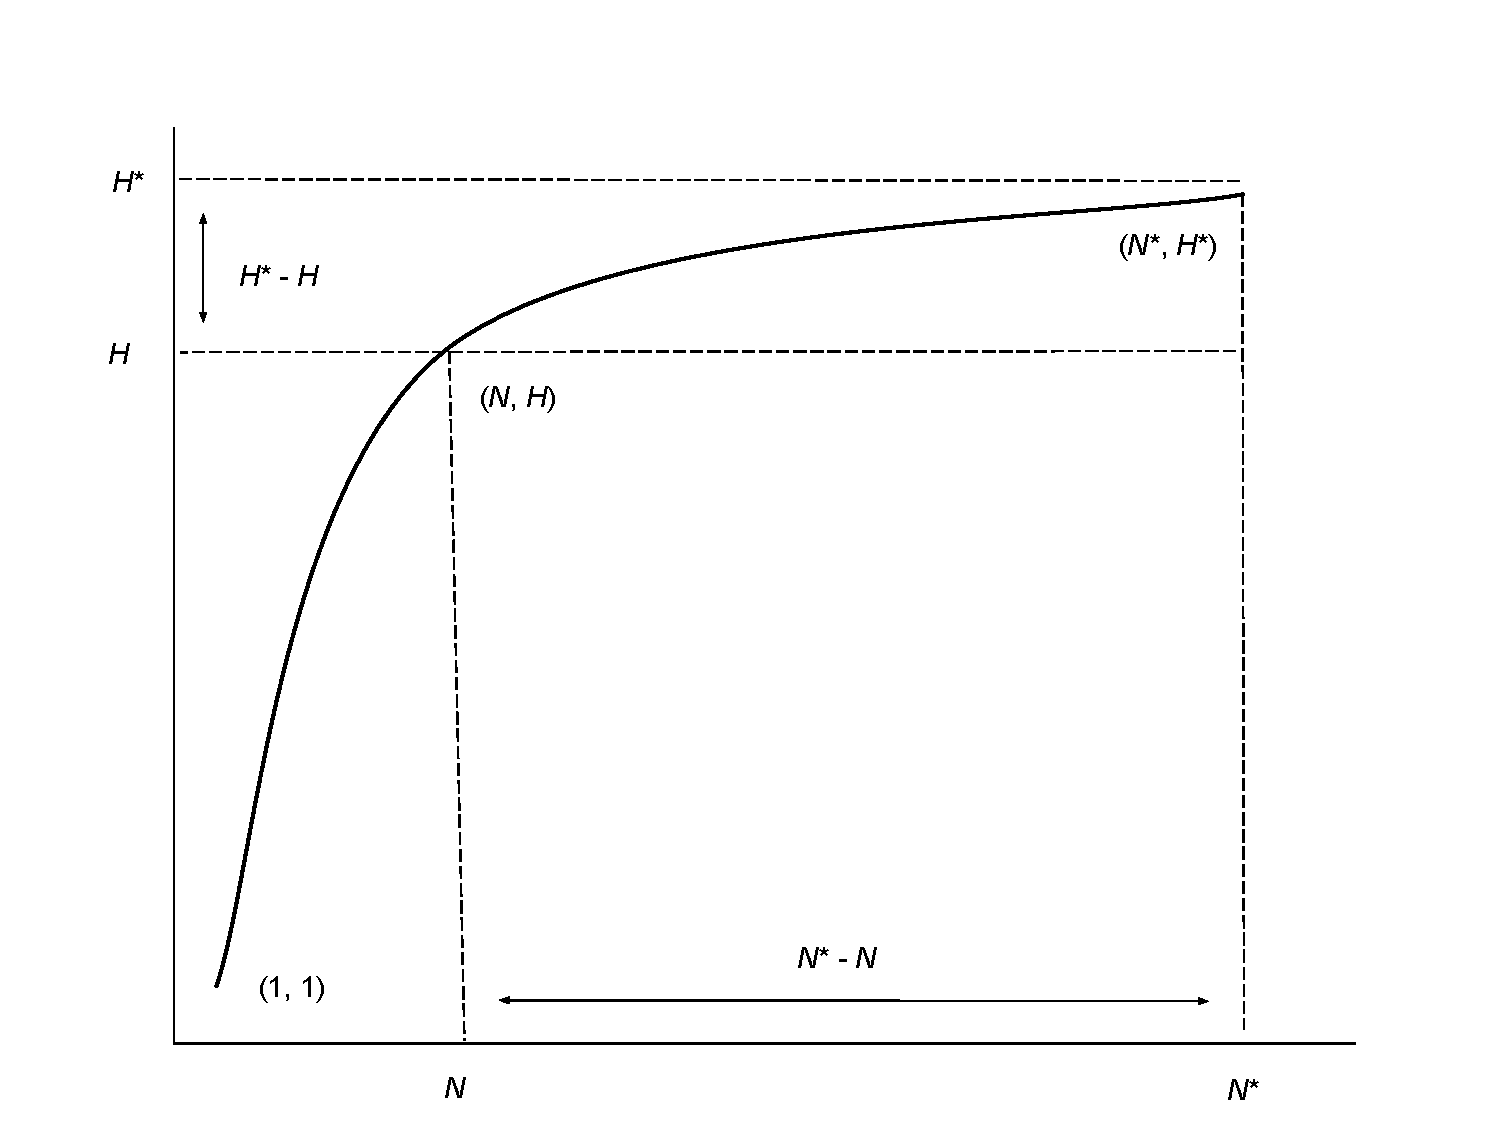
\includegraphics[width=0.8\textwidth]{Graph}
\caption[Visualization of Phillips \textit{et al.}'s \cite{phillips2015exploration} sampling model.]{Graphical depiction of Phillips \textit{et al.}'s \cite{phillips2015exploration} sampling model as described in detail within the main text. The \textit{x}-axis is meant to depict the number of specimens sampled, whereas the \textit{y}-axis is meant to convey the cumulative number of unique haplotypes uncovered for every additional individual that is randomly sampled. $N$ and $H$ refer to specimen and haplotype numbers that are observed for a given species. \textit{N}* is the total sample size that is needed to capture all \textit{H}* haplotypes that exist for a species.}
\end{figure}


\noindent \textbf{Figure 2.2} resembles the general shape of a saturated haplotype accumulation curve for a hypothetically well-sampled species. The point labelled ($N$, $H$) on the curve reflects the current level of sampling effort that has been expended for a given species (\textit{i.e.}, as found in BOLD). The goal is to extrapolate the curve to the point ($N^*$, $H^*$) to observe the value on the \textit{x}-axis (\textit{i.e., N}*) at which levelling off toward an asymptote (on the \textit{y}-axis) first becomes evident (\textit{i.e.}, at the value of \textit{H}*). Here, $N^*-N$ is the number of additional specimens that must be randomly sampled to observe $H^*-H$ additional haplotypes for a given species. If $H$ is equal to \textit{H}*, then \textit{N}* will be equal to $N$, and no further sampling is necessary; otherwise, if $H$ is less than \textit{H}*, then \textit{N}* will be greater than $N$, and additional sampling will be required.  The curve in \textbf{Figure 2.2} passes through the point (1, 1), which is due to the fact that the sampling of a single individual of a given species corresponds to observing one unique haplotype for that species.



\subsection{Application to Ray-finned Fishes}

Phillips \textit{et al.} \cite{phillips2015exploration} investigated levels of existing COI haplotype variation in 18 species of ray-finned fishes (Chordata: Actinopterygii) represented by a minimum of 60 individuals in accordance with Grewe \textit{et al.} \cite{grewe1993mitochondrial}. Results showed that 147-5379 specimens likely must be randomly sampled to uncover all predicted haplotype diversity in the selected species (between 3-528 total haplotypes) \cite{phillips2015exploration}. Sample size estimates obtained by Phillips \textit{et al.} \cite{phillips2015exploration} are comparable in magnitude to those of Zhang \textit{et al.} \cite{zhang2010estimating}, but not in the case of Luo \textit{et al.} \cite{luo2015simulation}, which are closer to practical sample sizes for DNA barcoding. Further, haplotype accumulation curves displayed evidence of reaching an asymptote for only 3/18 examined species: Chinook salmon (\textit{Oncorhynchus tshawytscha}), Rockfish (\textit{Sebastes} sp.) and Siamese fighting fish (\textit{Betta splendens}) based on significance testing of curve slopes with a one-sided \textit{t}-test using the last 10 points on the end of accumulation curves \cite{phillips2015exploration}. Of note is the haplotype accumulation curve for Chinook salmon, which appeared to show premature saturation despite only 12 out of an estimated total of 78 haplotypes being found for the species. At the time of publication of Phillips \textit{et al.}'s \cite{phillips2015exploration} study, \textit{Sebastes} sp. was linked to a single BIN. The BIN system is inherently dynamic: as more sequences are added within BOLD, specimens assigned to a single BIN may be allocated to multiple BINs or multiple existing BINs may be coalesced into a single BIN. This is especially the case as species boundaries become clearer or taxonomic revisions are made. As an example, the genus \textit{Sebastes} is a highly speciose group, thought to have undergone an adaptive radiation as recently as 8-9 million years ago \cite{steinke2009dna}. This fact could explain the low haplotype diversity observed for this species (two haplotypes across 98 individuals). Such findings may be due to the underlying assumptions of the model, which are likely to be over-simplistic, particularly that of equality of intraspecific haplotype frequencies. Further, the proposed estimator for the calculation of total haplotype diversity (\textit{H}*) (Equation 6) may be a gross overestimate. Despite not being realistic for populations of real species, the reason for adopting a uniform distribution of haplotypes was due to mathematical convenience, to make calculations of sample size as simple and as straightforward as possible. This is commonly done in practice, since determining the true distribution of species haplotypes is likely strongly dependent on species under study. Thus, values of \textit{N}* are likely overestimates of the true number of specimens that must be randomly sampled to observe most haplotype variation that exists for a species \cite{phillips2015exploration}. Phillips \textit{et al.} \cite{phillips2015exploration} argue that the use of a limited number of points in the calculation of curve slopes may not be adequate; the authors argue that a fixed proportion of curve points should instead be used. Further, through successively targeting the last 20-15\%, 15-10\% and the last 10\% of species haplotype accumulation curves, to observe a statistically-significant change in slope values, the precise point of saturation can be localized \cite{phillips2015exploration}.



Determining the precise point corresponding to haplotype accumulation curves \\ reaching an asymptote (\textit{i.e.}, having a slope near zero) is difficult. One way this can be accomplished is through employing numerical techniques, specifically iteration. Such methods work by repeatedly recycling computed values into an algorithm; that is, current values are used as starting values to the next iteration until convergence to a solution is achieved. One way this can be realized is through iterating Equation (7) along with the equations for the ``measures of sampling closeness'' proposed by Phillips \textit{et al.} \cite{phillips2015exploration}. This seems to be the most logical way forward in better ascertaining at what level specimen sampling is deemed sufficient and thus, when further collection of specimens should be ceased.

\section{Future Prospects}


This chapter explores the issue of sampling in DNA barcoding from the perspective of computational and statistical methodologies. Key sample size studies in the barcoding literature were examined in detail. A lack of consensus exists in the most appropriate number of specimens that must be targeted to uncover the majority of haplotype diversity that exists at the species level for a variety of taxa. This question is similar to the problem of calculating species divergence thresholds for taxon delimitation and is strongly dependent on species abundances, life histories and geographic coverage. To date, few studies \\ exploring sample sizes for DNA barcoding have been conducted. Existing studies (\cite{phillips2015exploration, zhang2010estimating}) appear to point to the comprehensive sampling of hundreds to thousands of specimens to capture a wide range of standing genetic variation for a given species based on \\ asymptotic behaviour of haplotype accumulation curves.



To thoroughly examine the issue of determining specimen sample sizes that are \\ necessary for full assessment of COI DNA barcode haplotype sampling completeness \\ within animal species, relaxation of assumptions inherent in Phillips \textit{et al.}'s \cite{phillips2015exploration} sampling model is necessary. Specifically, subsequent approaches should investigate the following:

\begin{enumerate}

\item relaxing the assumption of uniformity of species haplotype frequencies;

\vspace{1mm}

\item loosening the assumption of panmixia within species; and,

\vspace{1mm}

\item testing both above assumptions in tandem.

\end{enumerate}

\noindent The incorporation of population structure into models of haplotype sampling is not \\ straightforward, as sampling strategies for DNA barcoding are quite variable and highly dependent on the taxa under study. Thus, this necessitates the introduction of a more spatially-explicit systematic sampling (\textit{e.g.}, phylogeographic) of species genetic variation across distinct taxon boundaries and along phenotypic gradients (\textit{i.e.}, clines). The view of DNA barcoding metaphorically as a ``molecular transect", along which a wide range of intraspecific haplotype diversity can be uncovered, is fitting. Within-species genetic variation has been limited to over-representation of deep sampling of a single or a few populations. If the ultimate goal is to account for levels of standing genetic variation with species, then constraining taxon sampling to narrow geographic regions is not ideal, as this can be considered a form of pseudo-replication. This seems to be an issue of nestedness in sampling and while some depth of sampling within a population is certainly warranted, it cannot be conflated with depth of sampling across populations within a species. In addition, future research should aim to answer the question: is there an optimal threshold for specimen sampling above which no new DNA barcode haplotype variation is likely to be observed for a species? While it should be possible to find this limit for already well-sampled taxa based on trends seen in haplotype accumulation curves, the use of haplotype accumulation curves to estimate sample sizes that are required for full \\ assessment of COI DNA barcode haplotype sampling completeness has only been tested in one previous study (Zhang \textit{et al.} \cite{zhang2010estimating}). Phillips \textit{et al.} \cite{phillips2015exploration} expanded on previous studies through proposing a simple and easily implemented method to estimate specimen sample sizes for a number of ray-finned fish species, which are among the most densely sampled to date within BOLD. Sample size optimization for the identification of animal species across wide-ranging geographic scales is key since intraspecific variation within DNA barcodes is not easy to measure, and obtaining large numbers of barcodes that reflect a wide range of intraspecific genetic divergence is sometimes challenging \cite{bertolazzi2009learning}. In addition to being able to report likely required specimen sample sizes necessary to achieve saturation in species haplotype curves, it would be ideal if DNA barcoding studies could also provide a global measure of geographic dispersion to reliably test for cases of isolation-by-distance within species. Unfortunately, no such measure yet exists in this regard, making these kinds of analyses problematic. While model estimates may not be practical, having such a framework at hand that easily allows for the calculation of lower bounds for sample size offers researchers a glimpse into the most appropriate taxon sample sizes to target, and potentially where those taxa should be sampled. More crucially, the present simulation proposed herein can be employed to best determine the proper allocation of sampling effort, time and resources \cite{hortal2005ed}. Such work finds application in studies of metabarcoding \cite{wares2015can} as well as more broadly to global climate change \cite{pfenninger2012methodological}.


To thoroughly examine the issue of determining specimen sample sizes that are \\ necessary for full assessment of COI DNA barcode haplotype sampling completeness \\ within animal species, relaxation of assumptions inherent in Phillips \textit{et al.}'s \cite{phillips2015exploration} sampling model is necessary. Specifically, subsequent approaches should investigate the following:

\begin{enumerate}

\item relaxing the assumption of uniformity of species haplotype frequencies;

\vspace{1mm}

\item loosening the assumption of panmixia within species; and,

\vspace{1mm}

\item testing both above assumptions in tandem.

\end{enumerate}

\noindent The incorporation of population structure into models of haplotype sampling is not \\ straightforward, as sampling strategies for DNA barcoding are quite variable and highly dependent on the taxa under study. Thus, this necessitates the introduction of a more spatially-explicit systematic sampling (\textit{e.g.}, phylogeographic) of species genetic variation across distinct taxon boundaries and along phenotypic gradients (\textit{i.e.}, clines). The view of DNA barcoding metaphorically as a ``molecular transect", along which a wide range of intraspecific haplotype diversity can be uncovered, is fitting. Within-species genetic variation has been limited to over-representation of deep sampling of a single or a few populations. If the ultimate goal is to account for levels of standing genetic variation with species, then constraining taxon sampling to narrow geographic regions is not ideal, as this can be considered a form of pseudo-replication. This seems to be an issue of nestedness in sampling and while some depth of sampling within a population is certainly warranted, it cannot be conflated with depth of sampling across populations within a species. In addition,

\newpage

\section*{Acknowledgments}

We wish to greatly acknowledge the efforts of Rodger Gwiazdowski in providing \\ valuable edits to this manuscript. In addition, comments by Sarah (Sally) Adamowicz improved overall readability and flow of the manuscript considerably. Finally, two \\ anonymous revievers lent constructive feedback on this work, for which we are greatly appreciative.



This work was supported by a 2016/17 University of Guelph College of Physical and Engineering Science (CPES) Graduate Excellence Entrance Scholarship awarded to JDP.



The Dish With One Spoon Covenant speaks to our collective responsibility to steward and sustain the land and environment in which we live and work, so that all peoples, present and future, may benefit from the sustenance it provides. As we continue to strive to strengthen our relationships with and continue to learn from our Indigenous neighbours, we recognize the partnerships and knowledge that have guided the research conducted in our labs. We acknowledge that the University of Guelph resides in the ancestral and treaty lands of several Indigenous peoples, including the Attawandaron people and the Mississaugas of the Credit, and we recognize and honour our Anishinaabe, Haudenosaunee, and M{\'e}tis neighbours. We acknowledge that the work presented here has occurred on their traditional lands so that we might work to build lasting partnerships that respect, honour, and value the culture, traditions, and wisdom of those who have lived here since time immemorial.



\section*{Author Contributions}

JDP conducted the literature review and wrote the manuscript. DJG acted as an advisor in statistics. RHH acted as an advisor in DNA barcoding. All authors contributed to the revision of this manuscript and approved the final version. 



\section*{Conflict of Interest}

None declared.

Chapter 3

Earth is in the midst of its sixth mass extinction event and global biodiversity is \\ declining at an unprecedented rate \cite{ceballos2015accelerated}. It is therefore important that species genetic \\ diversity be catalogued and preserved. One solution to address this mounting crisis in a systematic, yet rapid way is DNA barcoding \cite{hebert2003biological}. DNA barcoding relies on variability within a small gene fragment from standardized regions of the genome to identify species, based on the fact that most species exhibit a unique array of barcode haplotypes that are more similar to each other than those of other species (\textit{e.g.}, a barcode ``gap"). In animals, the DNA barcode region corresponds to a 648 bp fragment of the 5' terminus of the cytochrome \textit{c} oxidase subunit I (COI) mitochondrial marker \cite{hebert2003biological, hebert2003barcoding}. A critical problem since the inception of DNA barcoding involves determining appropriate sample sizes necessary to capture the majority of existing intraspecific haplotype variation for major animal taxa \cite{hebert2004identification, meyer2005dna, ward2005dna}. Taxon sample sizes currently employed in practice for rapid assignment of a species name to a specimen, have ranged anywhere from 1-15 specimens per species \cite{goodall2012comparison, jin2012simple, matz2005likelihood, ross2008testing, yao2017evaluating}; however, oftentimes only 1-2 individuals are actually collected. This trend is clearly reflected within the Barcode of Life Data Systems (\href{http://www.boldsystems.org}{BOLD}) \cite{ratnasingham2007bold}, where an overwhelming number of taxa have only a single record and sequence.

 

A fitting comparison to the issue of adequacy of specimen sample sizes can be made to the challenge of determining suitable taxon distance thresholds for species separation on the basis of the DNA barcode gap \cite{meyer2005dna}. It has been widely demonstrated that certain taxonomic groups, such as Lepidoptera (butterflies/moths), are able to be readily separated into distinct clusters largely reflective of species boundaries derived using morphology \cite{candek2015dna}. However, adoption of a fixed limit of 2\% difference between maximum intraspecific distance and minimum interspecific (\textit{i.e}, nearest-neighbour) divergence is infeasible across all taxa \cite{collins2013seven, hebert2003barcoding}. Species divergence thresholds should be calculated from available \\ sequence data obtained through deep sampling of taxa across their entire geographic ranges whenever possible \cite{young2017barcode}. There is a clear relationship between specimen sample sizes and observed barcoding gaps: sampling too few individuals can give the impression of taxon separation, when in fact none exists \cite{candek2015dna, dasmahapatra2010mitochondrial, hickerson2006dna, meyer2005dna, wiemers2007does}, inevitably leading to erroneous conclusions \cite{collins2013seven}. It is thus imperative that barcode gap analyses be based on adequate sample sizes to minimize the presence of false positives. Introducing greater statistical rigour into DNA barcoding appears to be the clear way forward in this respect \cite{candek2015dna, luo2015simulation, nielsen2006statistical, phillips2019incomplete}. The introduction of computational approaches for automated species delimitation such as Generalized Mixed Yule Coalescent (GMYC) \cite{fujisawa2013delimiting, monaghan2009accelerated, pons2006sequence}, Automatic Barcode Gap Discovery (ABGD) \cite{puillandre2011abgd} and Poisson Tree Processes (PTP; \cite{zhang2013general}) has greatly \\ contributed to this endeavour in the form of web servers (\href{https://species.h-its.org/gmyc/}{GMYC}, \href{http://wwwabi.snv.jussieu.fr/public/abgd/abgdweb.html}{ABGD}, \href{https://species.h-its.org/ptp/}{PTP}) and R packages (GMYC: Species' LImits by Threshold Statistics, \href{https://r-forge.r-project.org/projects/splits/}{\tt splits} \cite{ezard2017splits}).



Various statistical resampling and population genetic methods, in particular coalescent simulations, for the estimation of sample sizes, have been applied to Lepidoptera (Costa Rican skipper butterflies (\textit{Astraptes fulgerator})) \cite{zhang2010estimating} and European diving beetles (\textit{Agabus bipustulatus}) \cite{bergsten2012effect}. Using Wright's equilibrium island model \cite{wright1951genetical} and Kimura's stepping stone model \cite{kimura1964stepping} under varying effective population sizes and migration rates, Zhang \textit{et al.} \cite{zhang2010estimating} found that between 156-1985 specimens per species were necessary to observe 95\% of all estimated COI variation for simulated specimens of \textit{A. fulgerator}. Conversely, real species data showed that a sample size of 250-1188 individuals is probably needed to capture the majority of COI haplotype variation existing for this species \cite{zhang2010estimating}. A subsequent investigation carried out by Bergsten \textit{et al.} \cite{bergsten2012effect} found that a random sample of 250 individuals was required to uncover 95\% COI diversity in \textit{A. bipustulatus}; whereas, a much smaller sample size of 70 specimens was necessary when geographic separation between two randomly selected individuals was maximized.

 

Others have employed more general statistical approaches. Based on extensive \\ simulation experiments, through employing the Central Limit Theorem (CLT), Luo \textit{et al.} \cite{luo2015simulation} suggested that no fewer than 20 individuals per species be sampled. Conversely, using an estimator of sample size based on the Method of Moments, an approach to parameter estimation relying on the Weak Law of Large Numbers \cite{pearson1894contributions}, sample sizes ranging from 150-5400 individuals across 18 species of ray-finned fishes (Chordata: Actinopterygii) were found by Phillips \textit{et al.} \cite{phillips2015exploration}.



Haplotype accumulation curves paint a picture of observed standing genetic variation that exists at the species level as a function of expended sampling effort \cite{phillips2019incomplete, phillips2015exploration}. \\ Haplotype sampling completeness can then be gauged through measuring the slope of the curve, which gives an indication of the number of new haplotypes likely to be uncovered with additional specimens collected. For instance, a haplotype accumulation curve for a hypothetical species having a slope of 0.01 suggests that only one previously unseen haplotype will be captured for every 100 individuals found. This is strong evidence that the haplotype diversity for this species has been adequately sampled. Thus, further recovery of specimens of such species provide limited returns on the time and money invested to sequence them. Trends observed from generated haplotype accumulation curves for the 18 actinopterygian species assessed by Phillips \textit{et al.} \cite{phillips2015exploration}, which were far from reaching an asymptote, corroborated the finding that the majority of intraspecific haplotypes remain largely unsampled in Actinopterygii for even the best-represented species in BOLD. \\ Estimates obtained from each of these studies stand in sharp contrast to sample sizes typically reported within DNA barcoding studies. 




For instance, due to evidence of sampling bias in otherwise densely-sampled taxa housed in BOLD (\textit{e.g.}, Lepidoptera), D'Ercole \textit{et al}. (J. D'Ercole, 2019, unpublished data) wished to assess whether or not intraspecific haplotype variation within butterfly species remains unsampled. To test this, the authors employed {\tt HACSim} to examine sampling comprehensiveness for species comprising a large barcode reference library for North American butterflies spanning 814 species and 14623 specimens.

\section{Results}

(\textbf{Fig. 3.8}). 


\begin{figure}[H]

\centering

\includegraphics[width=0.80\textwidth]{"Figure 8".png}

\caption[Haplotype frequency barplot for Lake whitefish (\textit{Coregonus clupeaformis}.]{Initial haplotype frequency distribution for $N$ = 235 high-quality lake whitefish (\textit{Coregonus clupeaformis}) COI barcode sequences obtained from BOLD. This species displays a highly-skewed pattern of observed haplotype variation, with Haplotype 1 accounting for \textit{c.} 91.5\% (215/235) of all sampled records.}

\end{figure}

\textbf{Fig. 3.11}). 


\begin{figure}[H]

\centering

\includegraphics[width=0.80\textwidth]{"Figure 11".png}

\caption[Haplotype frequency distribution for Deer tick (\textit{Ixodes scapularis}).]{Initial haplotype frequency distribution for $N$ = 349 high-quality deer tick (\textit{Ixodes scapularis}) COI barcode sequences obtained from BOLD. In this species, Haplotypes 1-8 account for \textit{c.} 51.3\% (179/349) of all sampled records.}


\end{figure}


\textbf{Fig. 3.14}).


\begin{figure}[H]

\centering

\includegraphics[width=0.80\textwidth]{"Figure 14".png}

\caption[Haplotype frequency distribution for Scalloped hammerhead (\textit{Sphyrna lewini}).]{Initial haplotype frequency distribution for $N$ = 171 high-quality scalloped hammerhead (\textit{Sphyrna lewini}) COI barcode sequences obtained from BOLD. In this species, Haplotypes 1-3 account for \textit{c.} 87.7\% (150/171) of all sampled records.}


\end{figure}
 

Algorithm output is shown below. 


\vspace{3mm}

\begin{figure}[H]

{\scriptsize \tt

\vspace{2mm}

{\noindent \#\# Set parameters for hypothetical species \#\#}

\vspace{1mm}

{\noindent > N <- 100 \# total number of sampled individuals} \\
{> Hstar <- 10 \# total number of haplotypes} \\
{> probs <- rep(1/Hstar, Hstar) \# equal haplotype frequency}

\vspace{2mm}

{\noindent \#\#\# Run simulations \#\#\#}

\vspace{1mm}

{\noindent > HACSObj <- HACHypothetical(N = N, Hstar = Hstar, probs = probs) \# call helper function}

\vspace{1mm}

{\noindent \# set seed here if desired, e.g., set.seed(12345)} \\
{> HAC.simrep(HACSObj)} 

\noindent Simulating haplotype accumulation...

\vspace{2mm}
 
\noindent |==============================================================================| 100\%
  
\vspace{3mm}
 
\noindent --- Measures of Sampling Closeness ---

\vspace{2mm} 
 
\noindent Mean number of haplotypes sampled:  10 \\
Mean number of haplotypes not sampled:  0 \\
Proportion of haplotypes sampled:  1 \\
Proportion of haplotypes not sampled:  0

\vspace{2mm} 
 
\noindent Mean value of N*:  100 \\
Mean number of specimens not sampled:  0

\vspace{3mm}
 
\noindent Desired level of haplotype recovery has been reached 

\vspace{3mm}

\noindent ---------- Finished. ----------
        
\noindent The initial guess for sampling sufficiency was N = 100 individuals
 
\noindent The algorithm converged after 1 iterations and took 3.637 s
 
\noindent The estimate of sampling sufficiency for p = 95\% haplotype recovery is N* = 100 \\ individuals ( 95\% CI: 100-100 )
 
\noindent The number of additional specimens required to be sampled for p = 95\% haplotype recovery \\ is N* - N = 0 individuals 

}

\end{figure}


\noindent The output of {\tt HACSim} is displayed below. 

\vspace{3mm}

\begin{figure}[H]

{\scriptsize \tt

{\noindent \#\#\# Run simulations \#\#\#}

\vspace{1mm}

{\noindent > HACSObj <- HACReal()}

\vspace{1mm}

{\noindent > HAC.simrep(HACSObj)} 

\vspace{1mm}

\noindent Simulating haplotype accumulation...

\vspace{2mm}
 
\noindent |==============================================================================| 100\%
  
\vspace{3mm}
 
\noindent --- Measures of Sampling Closeness ---

\vspace{2mm} 
 
\noindent Mean number of haplotypes sampled: 11.0705  \\
Mean number of haplotypes not sampled: 3.9295 \\
Proportion of haplotypes sampled: 0.7380333 \\
Proportion of haplotypes not sampled: 0.2619667   

\vspace{2mm} 
 
\noindent Mean value of N*: 318.4138 \\
Mean number of specimens not sampled: 83.4138

\vspace{3mm}
 
\noindent Desired level of haplotype recovery has not yet been reached 

\vspace{2mm}

\noindent |==============================================================================| 100\%

\vspace{3mm}

\noindent --- Measures of Sampling Closeness ---

\vspace{2mm} 
 
\noindent Mean number of haplotypes sampled: 13.8705  \\
Mean number of haplotypes not sampled: 1.1295 \\
Proportion of haplotypes sampled: 0.9247 \\
Proportion of haplotypes not sampled: 0.0753    

\vspace{2mm} 
 
\noindent Mean value of N*: 603.439 \\
Mean number of specimens not sampled: 45.43895

\vspace{3mm}
 
\noindent Desired level of haplotype recovery has not yet been reached

\vspace{2mm}

\noindent |==============================================================================| 100\%

\vspace{3mm}

\noindent --- Measures of Sampling Closeness ---

\vspace{2mm} 
 
\noindent Mean number of haplotypes sampled: 14.3708  \\
Mean number of haplotypes not sampled: 0.6292  \\
Proportion of haplotypes sampled:  0.9580533  \\
Proportion of haplotypes not sampled: 0.04194667    

\vspace{2mm} 
 
\noindent Mean value of N*: 630.4451  \\
Mean number of specimens not sampled: 26.44507

\vspace{3mm}
 
\noindent Desired level of haplotype recovery has been reached

\vspace{2mm}

\noindent ---------- Finished. ----------
        
\noindent The initial guess for sampling sufficiency was N = 235 individuals
 
\noindent The algorithm converged after 8 iterations and took 241.235 s 
 
\noindent The estimate of sampling sufficiency for p = 95\% haplotype recovery is N* = 604 \\ individuals ( 95\% CI: 601.504-606.496 )

\noindent The number of additional specimens required to be sampled for p = 95\% haplotype recovery \\ is N* - N = 369 individuals

}

\end{figure}



\noindent Simulation output of {\tt HACSim} is depicted below.

\vspace{3mm}

\begin{figure}[H]

{\scriptsize \tt

{\noindent \#\#\# Run simulations \#\#\#}

\vspace{1mm}

{\noindent > HACSObj <- HACReal()}

\vspace{1mm}

{\noindent > HAC.simrep(HACSObj)} 

\vspace{1mm}

\noindent Simulating haplotype accumulation...

\vspace{2mm}
 
\noindent |==============================================================================| 100\%
  
\vspace{3mm}
 
\noindent --- Measures of Sampling Closeness ---

\vspace{2mm} 
 
\noindent Mean number of haplotypes sampled: 65.3514  \\
Mean number of haplotypes not sampled: 17.6486   \\
Proportion of haplotypes sampled: 0.7873663 \\
Proportion of haplotypes not sampled: 0.2126337   

\vspace{2mm} 
 
\noindent Mean value of N*: 443.2499  \\
Mean number of specimens not sampled: 94.24988

\vspace{3mm}
 
\noindent Desired level of haplotype recovery has not yet been reached 

\vspace{2mm}

\noindent |==============================================================================| 100\%

\vspace{3mm}

\noindent --- Measures of Sampling Closeness ---

\vspace{2mm} 
 
\noindent Mean number of haplotypes sampled: 78.3713 \\
Mean number of haplotypes not sampled: 4.6287  \\
Proportion of haplotypes sampled: 0.9442325  \\
Proportion of haplotypes not sampled: 0.05576747     

\vspace{2mm} 
 
\noindent Mean value of N*: 802.7684  \\
Mean number of specimens not sampled: 44.76836

\vspace{3mm}
 
\noindent Desired level of haplotype recovery has not yet been reached

\vspace{2mm}

\noindent |==============================================================================| 100\%

\vspace{3mm}

\noindent --- Measures of Sampling Closeness ---

\vspace{2mm} 
 
\noindent Mean number of haplotypes sampled: 79.2147  \\
Mean number of haplotypes not sampled: 3.7853 \\
Proportion of haplotypes sampled: 0.954394 \\
Proportion of haplotypes not sampled: 0.04560602  

\vspace{2mm} 
 
\noindent Mean value of N*: 841.3716 \\
Mean number of specimens not sampled: 38.37161 

\vspace{3mm}
 
\noindent Desired level of haplotype recovery has been reached

\vspace{2mm}

\noindent ---------- Finished. ----------
        
\noindent The initial guess for sampling sufficiency was N = 349 individuals
 
\noindent The algorithm converged after 8 iterations and took 1116.468 s 
 
\noindent The estimate of sampling sufficiency for p = 95\% haplotype recovery is N* = 803 \\ individuals ( 95\% CI: 801.551-804.449 )

\noindent The number of additional specimens required to be sampled for p = 95\% haplotype recovery \\ is N* - N = 454 individuals

}

\end{figure}


\noindent {\tt HACSim} results are displayed below.

\vspace{3mm}

\begin{figure}[H]

{\scriptsize \tt

{\noindent \#\#\# Run simulations \#\#\#}

\vspace{1mm}

{\noindent > HACSObj <- HACReal()}

\vspace{1mm}

{\noindent > HAC.simrep(HACSObj)} 

\vspace{1mm}

\noindent Simulating haplotype accumulation...

\vspace{2mm}
 
\noindent |==============================================================================| 100\%
  
\vspace{3mm}
 
\noindent --- Measures of Sampling Closeness ---

\vspace{2mm} 
 
\noindent Mean number of haplotypes sampled: 9.9099  \\
Mean number of haplotypes not sampled: 2.0901  \\
Proportion of haplotypes sampled: 0.825825 \\
Proportion of haplotypes not sampled: 0.174175     

\vspace{2mm} 
 
\noindent Mean value of N*: 207.0657  \\
Mean number of specimens not sampled: 36.06566

\vspace{3mm}
 
\noindent Desired level of haplotype recovery has not yet been reached 

\vspace{2mm}

\noindent |==============================================================================| 100\%

\vspace{3mm}

\noindent --- Measures of Sampling Closeness ---

\vspace{2mm} 
 
\noindent Mean number of haplotypes sampled: 11.3231  \\
Mean number of haplotypes not sampled: 0.6769  \\
Proportion of haplotypes sampled: 0.9435917  \\
Proportion of haplotypes not sampled: 0.05640833      

\vspace{2mm} 
 
\noindent Mean value of N*: 413.3144 \\
Mean number of specimens not sampled: 23.31438

\vspace{3mm}
 
\noindent Desired level of haplotype recovery has not yet been reached

\vspace{2mm}

\noindent |==============================================================================| 100\%

\vspace{3mm}

\noindent --- Measures of Sampling Closeness ---

\vspace{2mm} 
 
\noindent Mean number of haplotypes sampled: 11.4769  \\
Mean number of haplotypes not sampled: 0.5231  \\
Proportion of haplotypes sampled: 0.9564083 \\
Proportion of haplotypes not sampled: 0.04359167    

\vspace{2mm} 
 
\noindent Mean value of N*: 432.8695 \\
Mean number of specimens not sampled: 18.8695 

\vspace{3mm}
 
\noindent Desired level of haplotype recovery has been reached

\vspace{2mm}

\noindent ---------- Finished. ----------
        
\noindent The initial guess for sampling sufficiency was N = 171 individuals
 
\noindent The algorithm converged after 9 iterations and took 174.215 s 
 
\noindent The estimate of sampling sufficiency for p = 95\% haplotype recovery is N* = 414 \\ individuals ( 95\% CI: 411.937-416.063 )

\noindent The number of additional specimens required to be sampled for p = 95\% haplotype recovery \\ is N* - N = 243 individuals

}

\end{figure}

\section{Discussion}

\subsection{Initializing {\tt HACSim} and Overall Algorithm Behaviour}

The overall stochastic behaviour of {\tt HACSim} is highly dependent on the number of \\ permutations used upon algorithm initialization. Provided that the value assigned to the {\tt  perms} argument is set high enough, numerical results ouputted by {\tt HACSim} will be found to be quite consistent between consecutive runs whenever all remaining parameter values remain unchanged. It is crucial that {\tt perms} not be set to too low a value to prevent the algorithm from getting stuck at local maxima and returning suboptimal solutions. This is a common situation with popular optimization algorithms such as hill-climbing. Attention therfore must be paid to avoid making generalizations based on algorithm performance and obtained simulation results \cite{spall2012stochastic}.



In applying the present method to simulated species data, it is important that selected simulation parameters are adequately reflective of those observed for real species. Thus, initial sample sizes should be chosen to cover a wide range of values based on those currently observed within BOLD. Such information can be gauged through examining species lists associated with BOLD records, which are readily accessible through Linnean search queries within the Taxonomy browser.



As with any iterative numerical algorithm, selecting good starting guesses for \\ initialization is key. While {\tt HACSim} is globally convergent (\textit{i.e.}, convergence is guaranteed for any value of $N \geq$ \textit{H}*), a good strategy when simulating hypothetical species is to start the algorithm by setting $N$ = \textit{H}*. In this way, the observed fraction of haplotypes found, $R$, will not exceed the desired level of haplotype recovery $p$, and therefore lead to overestimation of likely required specimen sample sizes. Setting $N$ high enough will almost surely result in $R$ exceeding $p$. Thus, arbitrarily large values of $N$ may not be biologically meaningful or practical. However, in the case of hypothetical species \\ simulation, should initial sample sizes be set too high, such that $R > p$, a straightforward workaround is to observe where the dashed horizontal line intersects the final haplotype accumulation curve (\textit{i.e.}, not the line the touches the curve endpoint). The resulting value of $N$ at this point will correspond with $p$ quite closely. This can be seen in \textbf{Fig. 5}, where an eyeball guess just over \textit{N}* = 20 individuals is necessary to recover $p$ = 95\% haplotype variation. A more reliable estimate can be obtained through examining the dataframe ``d'' outputted once the algorithm has halted (via {\tt envr\$d}). In this situation, simply look in the row corresponding to $p$\textit{H}* $\geq$ 0.95(10) $\geq$ 9.5. The required sample size is the value given in the first column ({\tt specs}). This is accomplished via the R code \\ {\tt envr\$d[which(envr\$d\$means $>=$ envr\$p * envr\$Hstar), ][1, 1]}.



The novelty of {\tt HACSim} is that it offers a systematic means of estimating likely \\ specimen sample sizes required to assess intraspecific haplotype diversity for taxa within large-scale genomic databases like GenBank and BOLD. Estimates of sufficient sampling suggested by our algorithm can be employed to assess barcode coverage within existing reference sequence libraries and campaign projects found in BOLD. Because  our method is the first to estimate likely required specimen sample sizes for species of interest, it is not yet possible to compare it to other algorithms meant for this purpose. Despite this, we anticipate that {\tt HACSim} will nevertheless provide regulatory applications with an unprecedented view and greater understanding of the state of standing genetic diversity (or lack thereof) within species.    



\subsection{Additional Capabilities and Extending Functionality of \tt{HACSim}}

In this chapter, we illustrate the application of haplotype accumulation curves to the broad assessment of species-level genetic variation. However, {\tt HACSim} is quite flexible in that one can easily explore likely required sample sizes at higher taxonomic levels (\textit{e.g.} order, family, genus) or specific geographic regions (\textit{e.g.}, salmonids of the Great Lakes) with ease. Such applicability will undoubtedly be of interest at larger scales (\textit{i.e.}. entire genomic sequence libraries). 



We foresee use of {\tt HACSim} being widespread within the DNA barcoding community. As such, improvements to existing code in terms of further optimization and algorithm runtime, as well as implementation of new methods by experienced R programmers in the space of DNA-based taxonomic identification, seems bright.



Potential extensions of our algorithm include support for the exploration of genetic variation at the Barcode Index Number (BIN) level \cite{ratnasingham2013dna}, as well as high-throughput sequencing (HTS) data for metabarcoding and environmental DNA (eDNA) applications. Such capabilities are likely to be challenging to implement at this stage until robust \\ operational taxonomic unit (OTU) clustering algorithms are developed (preferably in R). One promising tool in this regard for barcoding of bulk samples of real species and mock communities of known species composition is JAMP (\textbf{J}ust \textbf{A}nother \textbf{M}etabarcoding \\ \textbf{P}ipeline) devised for use in R by Elbrecht and colleagues \cite{elbrecht2018estimating}. JAMP includes a sequence read denoising tool that can be used to obtain haplotype numbers and frequency information (\textit{H}* and {\tt probs}). However, because JAMP relies on third-party software (particularly USEARCH \cite{edgar2010search} and VSEARCH \cite{rognes2016versatile}), it cannot be integrated within {\tt HACSim} itself and will thus have to be used externally. In extending {\tt HACSim} to next-generation space, two issues arise. First, it is not immediately clear how the argument $N$, is to be handled since multiple reads could be associated with single individuals. That is, unlike in traditional Sanger-based sequencing, there is not a one-to-one correspondence between specimen and sequence \cite{adams2019beyond, wares2015can}. Second, obtaining reliable haplotype information from noisy HTS datasets is challenging without first having strict quality filtering criteria in place to \\ minimize the occurrence of rare, low-copy sequence variants which may reflect artifacts stemming from the Polymerase Chain Reaction (PCR) amplification step or sequencing process \cite{braukmann2019metabarcoding, elbrecht2018estimating, turon2019metaphylogeography}. Turning to molecular population genetics theory might be the answer \cite{adams2019beyond}. Wares and Pappalardo \cite{wares2015can} suggest three different approaches to estimating the number of specimens of a species that may have contributed to a metabarcoding sample: (1) use of prior estimates of haplotype diversity, together with observed number of haplotypes; (2) usage of Ewens' sampling formula \cite{ewens1972sampling} along with estimates of Watterson's $\theta$ (not to be confused with the $\theta$ denoting true sampling sufficency herein) \cite{watterson1975segregating}, as well as total number of sampled haplotypes; and (3) employment of an estimate of $\theta$ and the number of observed variable sites ($S$) within a multiple sequence alignment. A direct solution we propose might be to use sequencing coverage/depth (\textit{i.e.}, the number of sequence reads) as a proxy for number of individuals. The outcome of this would be an estimate of the mean/total number of sequence reads required for maximal haplotype recovery. However, the use of read count as a stand-in for number of specimens sampled would require the unrealistic assumption that all individuals (\textit{i.e.}, both alive and dead) shed DNA into their environment at equal rates. The obvious issue with extending {\tt HACSim} to handle HTS data is computing power, as such data typically consists of millions of reads spanning multiple gigabytes of computer memory.



\subsection{Summary}

Here, we introduced a new statistical approach to assess specimen sampling depth within species based on existing gene marker variation found in public sequence databanks such as BOLD and GenBank. {\tt HACSim} is both computationally efficient and easy to use. We show utility of our proposed algorithm through both hypothetical and real species genomic sequence data. For real species (here, lake whitefish, deer tick and scalloped hammerhead), results from {\tt HACSim} suggest that comprehensive sampling for species comprising large barcode libraries within BOLD, such as Actinopterygii, Arachnida and Elasmobranchii is far from complete. With the availability of {\tt HACSim}, appropriate \\ sampling guidelines based on the amount of potential error one is willing to tolerate can now be established. For the purpose of addressing basic questions in biodiversity science, the employment of small taxon sample sizes may be adequate; however, this is not the case for regulatory applications, where greater than 95\% coverage of intraspecific haplotype variation is needed to provide high confidence in sequence matches defensible in a court of law.

     

Of immediate interest is the application of our method to other ray-finned fishes, as well as other species from deeply inventoried taxonomic groups such as Elasmobranchii (\textit{e.g.} sharks), Insecta (\textit{e.g.} Lepidoptera, Culicidae (mosquitoes)), Arachnida (\textit{e.g.}, ticks) and Chiroptera (bats) that are of high conservation, medical and/or socioeconomic importance. Although we explicitly demonstrate the use of {\tt HACSim} through employing COI, it would be interesting to extend usage to other barcode markers such as the \\ ribulose-1,5-bisphosphate carboxylase/oxygenase large subunit (rbcL) and maturase K \\ (matK) chloroplast genes for land plants, as well as the nuclear internal transcribed spacer (ITS) marker regions for fungi. The application of our method to non-barcode genes routinely employed in specimen identification like mitochondrial cytochrome \textit{b} (cyt\textit{b}) in birds for instance \cite{baker2009countering, lavinia2016calibrating}, nuclear rhodopsin (rho) for marine fishes \cite{hanner2011dna} or the \\ phosphoenolpyruvate carboxykinase (PEPCK) nuclear gene for bumblebees \cite{williams2015genes} is also likely to yield interesting results since sequencing numerous individuals at several different genomic markers can often reveal evolutionary patterns not otherwise seen from employing a single-gene approach (\textit{e.g.}, resolution of cryptic species or confirmation/revision of \\ established taxonomic placements) \cite{williams2015genes}. 



While it is reasonable that {\tt HACSim} can be applied to genomic regions besides 5'-COI, careful consideration of varying rates of molecular evolution within rapidly-evolving gene markers and the effect on downsteam inferences is paramount, as is sequence quality. Previous work in plants (Genus: \textit{Taxus}) by Liu \textit{et al.} \cite{liu2012sampling} has found evidence of a \\ correlation between mutation rate and required specimen sampling depth: genes evolving at faster rates will likely require larger sample sizes to estimate haplotype diversity compared to slowly-evolving genomic loci. We simply focused on 5'-COI because it is by far the most widely sequenced mitochondrial locus for specimen identification, owing to its desirable biological properties as a DNA barcode for animal taxa and because it has an associated data standard to help filter out poor-quality data \cite{phillips2019incomplete}. However, it should be noted that species diagnosis using COI and other barcode markers is not without its challenges. While COI accumulates variation at an appreciable rate, certain taxonomic groups are not readily distinguished on the basis of their DNA barcodes (\textit{e.g.}, the so-called ``problem children'', such as Cnidaria, which tend to lack adequate sequence divergence \cite{bucklin2011dna}). Other taxa, like Mollusca, are known to harbour indel mutations \cite{layton2014patterns}. Introns within Fungi greatly complicate sequence alignment \cite{min2007assessing}. Thus, users of {\tt HACSim} must exercise caution in interpreting end results with other markers, particularly those which are not protein-coding.



It is necessary to consider the importance of sampling sufficiency as it pertains to \\ the myriad regulatory applications of specimen identification  established using DNA \\ barcoding (\textit{e.g.}, combatting food fraud) in recent years. It since has become apparent that the success of such endeavours is complicated by the ever-evolving state of public reference sequence libraries such as those found within BOLD, in addition to the the inclusion of questionable sequences and lack of sufficent metadata for validation purposes in other genomic databases like GenBank (\textit{e.g.}, \cite{harris2003can}). Dynamic DNA-based identification systems may produce multiple conflicting hits to otherwise corresponding submissions over time. This unwanted behaviour has led to a number of regulatory agencies creating their own \textit{static} repositories populated with expertly-identified sequence records tied to known voucher specimens deemed fit-for-purpose for molecular species diagnosis and forensic compliance (\textit{e.g.} the United States Food and Drug Administration (USFDA)'s Reference Standard Sequence Library (\href{https://www.accessdata.fda.gov/scripts/fdcc/?set=seafood_barcode_data}{RSSL}) employed to identify unknown seafood samples from species of high socioeconomic value). While such a move has partially solved the problem of dynamism inherent in global sequence databases, there still remains the issue of low sample sizes that can greatly inflate the perception of barcode gaps between species. \\ Obtaining adequate representation of standing genetic variation, both within and between species, is therefore essential to mitigating false assignments using DNA barcodes. To this end, we propose the use of {\tt HACSim} to assess the degree of saturation of haplotype accumulation curves to aid regulatory scientists in rapidly and reliably projecting likely sufficient specimen sample sizes required for accurate matching of unknown queries to known Linnean names.



A defining characteristic of {\tt HACSim} is its convergence behaviour: the method \\ converges to the desired level of haplotype recovery $p$ for any initial guess $N$ specified by the user. Based on examples explored herein, it appears likely that already-sampled species within repositories like BOLD are far from being fully characterized on the basis of existing haplotype variation. In addition to this, it is important to consider the current limitations of our algorithm. We can think of only one: it must be stressed that appropriate sample size trajectories are not possible for species with only single representatives within public DNA sequence databases because haplotype accumulation is unachievable with only one DNA sequence and/or a single sampled haplotype. Hence, {\tt HACSim} can only be applied to species with at least two sampled specimens. Thus, application of our method to assess necessary sample sizes for full capture of extant haplotype variation in exceedingly rare or highly elusive taxa is not feasible. Despite this, we feel that {\tt HACSim} can greatly aid in accurate and rapid barcode library construction necessary to thoroughly appreciate the diversity of life on Earth.


\newpage

\section*{Acknowledgments}

The authors wish to extend thanks to Robert (Rob) Young for helpful discussions and providing critical feedback on an earlier draft of this manuscript that greatly improved its flow and overall readability.

 

This work was supported by a University of Guelph College of Physical and \\ Engineering Science (CPES) Graduate Excellence Entrance Scholarship awarded to JDP.



The Dish With One Spoon Covenant speaks to our collective responsibility to steward and sustain the land and environment in which we live and work, so that all peoples, present and future, may benefit from the sustenance it provides. As we continue to strive to strengthen our relationships with and continue to learn from our Indigenous neighbours, we recognize the partnerships and knowledge that have guided the research conducted in our labs. We acknowledge that the University of Guelph resides in the ancestral and treaty lands of several Indigenous peoples, including the Attawandaron people and the Mississaugas of the Credit, and we recognize and honour our Anishinaabe, Haudenosaunee, and M{\'e}tis neighbours. We acknowledge that the work presented here has occurred on their traditional lands so that we might work to build lasting partnerships that respect, honour, and value the culture, traditions, and wisdom of those who have lived here since time immemorial.



\section*{Author Contributions}

JDP conducted the literature review and wrote the manuscript. DJG acted as an advisor in statistics. RHH acted as an advisor in DNA barcoding. All authors contributed to the revision of this manuscript and approved the final version. 



\section*{Conflict of Interest}

None declared.



\section{Chapter 4}

\begin{figure}[H]

\centering

\includegraphics[width=0.80\textwidth]{"Fig. 1".png}

\caption[Initial haplotype frequency distribution for Pea aphid (\textit{Acyrthosiphon pisum}).]{Initial haplotype frequency distribution for $N$ = 356 high-quality Pea aphid (\textit{Acyrthosiphon pisum}) COI barcode sequences obtained from BOLD. This species displays a highly-skewed pattern of observed haplotype variation, Haplotype 1 accounts for \textit{c.} 96.6\% (344/356) of all sampled records.}

\end{figure}
 
\begin{figure}[H]

\centering

\includegraphics[width=0.80\textwidth]{"Fig. 2".png}

\caption[Initial haplotype frequency distribution for Common mosquito (\textit{Culex pipiens}).]{Initial haplotype frequency distribution for $N$ = 217 high-quality Common mosquito (\textit{Culex pipiens}) COI barcode sequences obtained from BOLD. In this species, Haplotype 1 accounts for \textit{c.} 84.3\% (183/217) of all sampled records.}

\end{figure}


\begin{figure}[H]

\centering

\includegraphics[width=0.80\textwidth]{"Fig. 3".png}

\caption[Initial haplotype frequency distribution for Gypsy moth (\textit{Lymantria dispar}).]{Initial haplotype frequency distribution for $N$ = 365 high-quality Gypsy moth (\textit{Lymantria dispar}) COI barcode sequences obtained from BOLD. In this species, Haplotypes 1-5 account for \textit{c.} 70.4\% (257/365) of all sampled records.}


\end{figure}



\section*{Supplemental Information}

Figures associated with running {\tt HACSim} with {\tt p} = 0.80 and {\tt p} = 0.90 for both \\ hypotetical and real species can be found on the primary author's GitHub repository \\ available at: https://github.com/jphill01/PhD-Thesis-Appendix.



\section*{Conflict of Interest}

None declared.



\section*{Acknowledgements}

We wish to thank Robert (Rob) Young for helpful discussions throughout this work.



We acknowledge that the University of Guelph resides on the ancestral lands of the Attawandaron people and the treaty lands and territory of the Mississaugas of the Credit. We recognize the significance of the Dish with One Spoon Covenant to this land and offer our respect to our Anishinaabe, Haudenosaunee and M{\'e}tis neighbours as we strive to strengthen our relationships with them.



\section*{Author Contributions}

JDP wrote the manuscript, approved all developed code as well as analyzed and \\ interpreted all experimental results. SEB wrote required code and performed all \\ experiments.  DJG acted as an advisor in statistics. RHH acted as an advisor in DNA barcoding. All authors contributed to the revision of this manuscript and approved the final version. 















































Chapter 4

DNA barcoding \cite{hebert2003biological} employs short, universal regions of genomic DNA, such as the \textit{c.} 648 bp fragment taken from the 5' end of the cytochrome \textit{c}. oxidase subunit I (COI) gene for animals \cite{hebert2003barcoding}, to readily identify unknown specimens to known species by matching queries to reference sequences housed in barcode libraries such as those found in the Barcode of Life Data Systems (BOLD; \cite{ratnasingham2007bold}; http://www.boldsystems.org) and GenBank. Early on, when DNA barcoding was first proposed,  estimates of sufficient sample sizes needed to recover levels of standing genetic variation within species of interest were often quite low and rather arbitrary, typically 20 or fewer specimens per species \cite{phillips2019incomplete, phillips2020hacsim, phillips2015exploration}. Even some early studies have expressed the need for more comprehensive sampling efforts \cite{zhang2010estimating}, but until now, a systematic approach was not available to provide optimal specimen sample sizes to adequately capture intraspecific DNA sequence variation. Such a tool is promising since required specimen sample sizes will vary considerably based on evolutionary history and life history of the species under consideration. For instance, different genomic marker loci evolve at different rates; thus, more rapidly evolving genes will likely require larger sample sizes compared to more slowly-evolving molecular loci \cite{phillips2019incomplete}. 



Recognizing this, in addition to plotting haplotype accumulation curves for a wide variety of ray-finned fishes (Chordata: Actinopterygii), \cite{phillips2015exploration} employed simple linear regression on the endpoints of accumulation curves to test the hypothesis that there was no evidence of additional haplotypes remaining to be sampled for a species. This was accomplished through testing that terminal curve slopes are equal to zero. Phillips \textit{et al.} \cite{phillips2015exploration} then calibrated their findings with a crude deterministic base model of likely required specimen sampling levels necessary to recover all estimated total haplotypes that might exist for a given species, grounded on the unrealistic assumption that species' haplotypes are sampled uniformly across known ecologic and geographic ranges. Estimates of \\ sampling sufficiency produced by Phillips \textit{et al.}'s \cite{phillips2015exploration} model are likely to be heavily biased due to the restrictive assumption of uniformity of species' haplotypes.


Their approach employs an initial guess of sampling sufficiency ($N$) to iteratively propose improving estimates of sample size necessary to capture a predefined minimum cutoff ({\tt p}), typically 95\%, of observed haplotype diversity for both hypothetical and real species based on a species' haplotype frequency distribution ({\tt probs}), \\ representing the probability of occurrence of each haplotype in a randomly-collected \\ specimen sample. A user need only additionally supply the number of permutations \\ ({\tt perms}) to be employed in the search, which acts to control both the \textit{numerical} accuracy and precision of computed sample size estimates by increasing or decreasing the \\ smoothness of the generated accumulation curve. Note here that improving the \textit{statistical} accuracy/precision of said estimates would require more specimens to be sampled.  Each randomly generated permutation represents a plausible assignment of species haplotypes to every sampled specimen. In simulating hypothetical species, \textit{H}* must be less than or equal to $N$ (this constraint is always satisfied for real species). The case of \textit{N} = \textit{H}*  corresponds to encountering a new, previously unseen species' haplotype for every additional specimen that is collected. For real species, $N$, \textit{H}* and {\tt probs} are calculated automatically from an imported FASTA file of aligned and trimmed single-marker DNA sequences.

Two important assumptions arise in considering the overall utility of {\tt HACSim} for assessing standing levels of genetic variation within species \cite{phillips2020hacsim}: 

\begin{enumerate}
\item that haplotypic variation observed in a randomly collected sample of specimens is representative of the true species' population (which is unknown \textit{a priori}); and,

\item that unsampled haplotypes are rare in a species' population (\textit{i.e.}, haplotypes occur at low frequency, potentially found in only 1-2 individuals -- otherwise they would have already been sampled).
\end{enumerate}

\noindent Assumption 1 is a common one adopted in many statistical resampling procedures such as nonparametric bootstrapping and is equivalent to treating a randomly drawn sample as if it were in fact the population of interest. Implicit in the present haplotype sampling model is the fact a randomly drawn sample of individuals makes up only a small fraction of the total species' population size. Assumption 2 is a strong, yet unrealistic one that is necessary within the framework of the underlying model. Whereas the total number of expected haplotypes that might exist for a given species' is readily estimated from observed data (such as through the Chao1 abundance estimator \cite{chao1984nonparametric}), the probabilities associated with unseen haplotypes cannot be known with absolute certainty \cite{phillips2020hacsim}. Therefore, the number of observed unique haplotypes for a species serves as a reasonable proxy for the total number of haplotypes that might exist for said species. In the context of the GSSSP investigated herein, Assumptions 1 and 2 together amount to assuming that all genetic diversity observed in reference sequence databases such as BOLD and related repositories arise from a single \textit{infinitely-large} panmictic (\textit{i.e.}, randomly-mating) species' population of constant size from which individuals are randomly sampled without replacement \\ \cite{phillips2015exploration}. That is, the current model underlying {\tt HACSim} disregards both the contribution of genetic drift which acts to alter haplotype frequencies in small species populations, as well as spatial effects which arise as a result of population substructuring via gene flow \cite{phillips2019incomplete}. It is recognized that the abovementioned assumptions will likely not be met for most real species. Violations of stated assumptions can only be mitigated through more thorough specimen sampling, and therefore further sampling of standing intraspecific haplotype variation. Extensions to {\tt HACSim}'s underlying sampling algorithm to better reflect true evolutionary dynamics at both the population and species levels have yet to be fully investigated.

When running simulations of real taxa obtained from reference sequence databases, the number of DNA sequences in a final single-species multiple sequence \\ alignment, the corresponding number of observed unique species' haplotypes, and the species' haplotype frequency distribution are all used for algorithm initialization. \\ Specifically, the iteration scheme used by {\tt HACSim} is

\begin{equation}
N^*_{i+1} = \frac{N_iH^*}{H_i}
\end{equation}

\noindent where $H_i$ is the cumulative mean number of observed unique species' haplotypes found from randomly sampling $N_i$ individuals at iteration $i$.

 

Drawing on the field of evolutionary computation, which is loosely based on Darwinian theory, $H_i$ can be likened to a fitness function that is to be maximized across all sampled specimens. Specifically, the ``fitness" function being optimized above is expressed \\ mathematically as

\begin{equation}
H_i = \left(\dfrac{1}{{\tt perms}}\sum_{k}{x_{jk}}\right)_{k=N}
\end{equation}

\noindent where $x_{jk}$ is a {\tt perms} $\times$ $N$ array, $j \in \{1, ..., {\tt perms}\}$ denotes array rows and $k \in \{1,...N\}$ references array columns. The array generated internally by {\tt HACSim} consists of positive integers in the range [1, \textit{H}*] that are drawn randomly according to {\tt probs}, a sorted vector of decreasing values between 0 and 1, whose elements must sum to 1. The filled population array forms the representation of solutions encoding the algorithm's search space. Elements within each row of the filled array are sampled according to {\tt probs}. That is, if, say, there are $N$ = 100 individuals and Haplotype 1 occurs at 90\% frequency, then approximately 90 individuals would be randomly assigned a label of 1. This scheme then continues for all remaining haplotypes.  Accumulation of unique species' haplotypes is then carried out through randomly sampling individual specimens (columns) of said array across all permutations (array rows). Cumulative means of the number of haplotypes recovered for each specimen, as per Equation (4.2), are then computed across all sampled permutations. The last array column corresponds to sampling $N$ individuals for a given species in Equation (4.2). Equation (4.1) produces a \\ monotonically-increasing and convergent sequence of estimates for sampling sufficiency even though the average number of species' haplotypes found at each iteration of {\tt HACSim} may fluctuate randomly; eventually, $H_i$ will approach \textit{H}* and therefore $N_i$ approaches \textit{N}*. {\tt HACSim} terminates when the observed proportion of haplotypes retrieved (\textit{R = $\frac{H_i}{H^*}$}) is at least {\tt p}. The rate of convergence of outputted haplotype accumulation curves to an asymptote depends highly on the value of {\tt perms}. When {\tt perms} is set high enough, the endpoint of the resulting curve, generated at each iteration of the algorithm, will be close in magnitude to the maximum value of the cumulative mean calculated across all columns of the constructed array. This behaviour provides a clear rationale for selection of the objective function being optimized herein. Further, the inclusion of a larger number of permutations acts to incorporate more diverse solutions into the search, while at the same time permitting {\tt HACSim}'s iterative search to ``hone in" on promising solutions through \\ exploitation/intensification of the problem space. Such behaviour is in sharp contrast to setting {\tt perms} to a small value, where {\tt HACSim} is reduced to searching the space of potential solutions randomly, while simultaneously performing a much broader search through exploration/diversification. Striking a careful balance between \\ exploration/diversification and exploitation/intensification is key to avoiding premature \\ algorithmic convergence and search efficiency issues. 

 

Estimates of sampling sufficiency ($\theta$) provided by {\tt HACSim} correspond to the point on the $x$-axis of haplotype accumulation curves where saturation of species genetic variation is likely to occur. Since one is interested in devising an optimal stopping rule for specimen sampling, it becomes necessary to closely monitor the endpoint of haplotype accumulation curves generated at each iteration of {\tt HACSim}'s run. A single run of {\tt HACSim} entails successively generating {\tt perms} accumulation curves internally and outputting a mean \\ curve at each iteration. Each successive iteration within a single run of {\tt HACSim} is an extrapolation of the curve generated in the preceeding iteration. The $x$-value corresponding to the point where the curve endpoint touches the horizontal line formed by the prespecified threshold for haplotype recovery is our best estimate of the sample size needed to fully characterize haplotype variation within a species, given current genomic data. 

Further, while there are numerous parameters that can be tweaked within {\tt HACSim} itself, a careful parameter sensitivity analysis is not the goal of the present study. This is not to say that altering either the number of permutations or the proportion of observed haplotype diversity to recover will produce unpredictable results. Clearly, increasing (decreasing) {\tt perms} results in increased (decreased) numerical \\ accuracy/precision of model estimates and smoother (noisier) haplotype accumulation \\ curves, while leading to slow (fast) computation. Similarly, increasing (decreasing) {\tt p} leads to higher (lower) estimates of sampling sufficiency (\textit{N}*), since more (fewer) species' haplotypes (\textit{i.e.}, higher (lower) $H_i$) need to be captured. Additionally, since specimen sample sizes are presumed to be strongly taxon-specific, due to differences in evolutionary origins and life history traits among species, and because {\tt HACSim} is meant to be a general modelling framework, it is highly unlikely that a single combination of {\tt perms} and {\tt p} can be found that works for the majority of taxa. Nevertheless, this should be explored in future work.


As such, this necessitates a brief discussion around {\tt HACSim}'s \textit{search space}.

\vspace{5mm}

\subsubsection{Theory}

A search space encompasses the domain over which a function is to be optimized \\ (\textit{i.e.}, either minimized or maximized) and includes all plausible solutions to said search problem. The search space explored by stochastic optimization algorithms can be best framed in the context of a person attempting to ascend to the top of hill or mountain. Said hill (or mountain) contains numerous peaks, plateaus and valleys, each with varying levels of steepness that together form a fitness landscape. The hill's (or mountain's) terrain is analogous to local optima encountered in an algorithmic search problem. In general, solving the GSSSP through pure brute force (\textit{i.e.}, exhaustive search) or random search is difficult owing to the size of the search space that must be explored: both specimen- and haplotype-level information need to be taken into account. Here, a (partial) solution to the GSSSP corresponds to the generation of a permutation. In the present work, the notion of a ``permutation" is distinct from the traditional mathematical meaning of the term. Within the field of combinatorics, a permutation is any (re)ordering of elements contained in a set. Herein, a random permutation appearing in the array generated by {\tt HACSim} according to some underlying probability distribution may comprise elements which are different from those appearing in any other permutation. For instance, one permutation of five specimens drawn from a uniform distribution over observed species' haplotypes labels may be given by the tuple (2, 1, 1, 5, 2), while another may be (5, 1, 3, 4, 4). ``Permutation" is used here to simply emulate terminology used in similar R packages that construct haplotype (and species) accumulation curves such as {\tt spider} \cite{brown2012spider} and {\tt vegan} \cite{dixon2003vegan}. Since {\tt HACSim} can be considered a population-based metaheuristic, the state space size explored would be \cite{chopard2018metaheuristics}

\begin{equation}
|S| = (H^*)^N.
\end{equation} 

\noindent Equation (4.3) above denotes the number of ways of assigning \textit{H}* haplotypes to $N$ \\ individuals \textit{with} replacement (\textit{i.e.}, repetition is permitted), and where the order in which haplotypes are allocated to specimens is important. Thus, the probability of reaching the global optimum once across the entire fitness landscape under random search (that is, selecting a candidate solution uniformly at random) is approximately given by

\begin{equation}
P(G) = \frac{1}{(H^*)^N}
\end{equation} 

\noindent where $G$ is defined as the event ``reaching the global optimum". Even for a ``reasonable" number of specimens and observed species' haplotypes typical of many taxon-focused DNA barcoding studies, the search space can become prohibitively large due to \\ fundamental biological processes and mechanisms underpinning the evolution of species (\textit{e.g.}, mutation). Therefore, in the case of the GSSSP, the fitness landscape is not guaranteed to be defined by a strictly unimodal hill/mountain. Typically, in most optimization \\ problems, several different potential solutions are tried in a systematic way, making a given future observation more likely to be the global optimum compared to earlier ones. Hence, the fraction of {\tt HACSim}'s search space traversed is $\frac{{\tt perms}}{|S|}$. For instance, via Equation (4.3) and Equation (4.4), the search space characterizing a species represented by $N = 100$ individuals and \textit{H}* = 10 unique haplotypes would contain $|S| = 10^{100}$ potential solutions where the probability of finding the globally optimal solution is only $P(G) = 10^{-100}$. Moreover, as with many other stochastic optimization algorithms, the size of the search space actually explored in a given run of {\tt HACSim} is exceedingly small.

\vspace{5mm}

It is important to realize that sample size estimates provided by {\tt HACSim} are strongly affected by parameters specific to algorithm tuning, particularly {\tt perms}. That is, it should be stressed that while {\tt HACSim} does indeed provide a convergence guarantee, it provides no guarantee of global optimality; the tool merely computes a ``good enough" (\textit{i.e.}, locally optimal) solution in a finite amount of computation time. Thus, solution quality is entirely dependent on the number of permutations a user deems approropriate for their species of interest and is willing to employ given computational power constraints, as well as tests of researchers' patience and sanity. Within {\tt HACSim}, {\tt perms} must be at least two to allow calculation of confidence interval (CI) estimates for generated curves; however, such a \\ permutation size is not sufficient. In general, it is advised that {\tt perms} be set to a ``large" value to minimize the effects of Monte Carlo sampling error through reducing the variance in resulting haplotype accumulation curves and their associated ``measures of sampling \\ closeness", as well as ensuring the search does not become trapped in local optima. When too few permutations are employed, {\tt HACSim} will tend to return estimates (\textit{N}*) equal to, or too close to, the initial guess ($N$) for sampling sufficiency. To avoid such behaviour, typically {\tt perms} is set to 10000 or higher, but this strongly affects algorithm runtime since more candidate solutions in the search space need to be enumerated \cite{phillips2020hacsim}. Even with a permutation size of 10000, only $\frac{10000}{10^{100}} = 10^{-94}\%$ of the entire search space for the example above is actively explored.

\vspace{5mm}

While there are $|S| = (H^*)^N$ possible orderings (or resamples) of all observed species' haplotypes to each collected specimen, a number of such orderings are equivalent, and thus redundant, under the exchangeability property of random variables \cite{chernick2011bootstrap}. That is, given two sequences of random variables having the exact same elements in common, their joint probability distribution is unchanged whenever elements in either sequence are reordered.  Hence, here, ordering of haplotypes to individual specimens is irrelevant, and, without proof (though easily proved with a direct algebraic proof, a combinatorial proof or mathematical induction; see \textbf{Appendix D} for details), the search space is considerably reduced to a size of

\begin{equation}
|S| = \multichoose{H^*}{N} = {{N + H^* - 1}\choose{N}} = {{N + H^* - 1}\choose{H^* - 1}} = \frac{(N + H^* - 1)!}{N!(H^* - 1)!}
\end{equation}

\noindent where $n! = \prod_{i=1}^n{i}$ ($n!$ read as ``$n$ factorial") expresses the number of permutations of $n$ distinct objects, and ${n}\choose{k}$ = $\frac{n!}{k!(n-k)!}$ is the binomial coefficient, denoting the number of ways to select $k$ unique objects from a total of $n$ \textit{without} replacement, neglecting the order in which objects are sampled. The quantity $\multichoose{k}{n}$ (read as ``$k$ multichoose $n$") represents the number of $n$-element multisets on a $k$-element set. Equation (4.5) above expresses the total number of ways to assign $N$ indistinguishable specimens to \textit{H}* distinguishable haplotypes \textit{with} replacement when the order in which haplotypes are drawn is unimportant. Such a scheme closely mirrors a classic urn sampling process seen in population genetics \\ (specifically, Coalescent theory \cite{kingman1982coalescent}) whereby distinctly-coloured marbles (or another similar entity such as balls) representing individual alleles are picked at random one at a time from one or several identical urns. The probability of attaining the global optimum within the reduced space is now

\begin{equation}
P(G) = \frac{1}{\multichoose{H^*}{N}} = \frac{1}{{{N + H^* - 1}\choose{N}}} = \frac{1}{{{N + H^* - 1}\choose{H^* - 1}}} = \frac{N!(H^* - 1)!}{(N + H^* - 1)!}
\end{equation}

\noindent Here, employing the same example discussed previously, the search space now comprises only $|S| = \multichoose{10}{100} = {{100 + 10 - 1}\choose{100}} = {{100 + 10 - 1}\choose{10 - 1}} = 4.26 \times 10^{12}$ possible solutions, and thus the probability of locating the global optimum is significantly higher at \\ $P(G) = 2.35 \times 10^{-13}$. Hence, given a permutation size of 10000, approximately \\ $2.35 \times 10^{-7}\%$ of the search space is systematically explored. Yet, for most real species, the reduced search space is still far too large to blindly explore; that is, random specimen sampling is no longer a feasible option.




The KW test extends the Mann-Whitney $U$ test (also known as the Wilcoxan Rank Sum test) to more than two groups. The $U$ test is the nonparametric version of the \\ two-independent-samples $t$ test. Performing successive pairwise $t$-tests on three or more groups is problematic. See the following paragraphs for more information. 



A brief discussion here of the problem of testing multiple statistical inferences \\ simultaneously is necessary. The issue at hand is that such a procedure will tend to inflate the Family-wise Error Rate (FWER). The FWER corresponds the Type I error rate, that is, the probability of rejecting the null hypothesis of no significant difference between groups when one in fact exists, given the null hypothesis is true, can be quite high. Because one of the present goals of this study is to assess significance at the 5\% level ($\alpha$ = 0.05, 95\% confidence) for $n$ = 6 distinct pairwise comparisons, the probability of committing a Type I error is FWER = $1 - (1 - \alpha)^n = 1 - (1-0.05)^6 \approx 0.265$. The FWER increases with larger values of $\alpha$ (smaller confidence levels). Fortunately, various methods have been proposed for controlling the FWER.

Herein, the Bonferroni correction is employed to minimize the risk of falsely rejecting a true null hypothesis. While conservative, Bonferroni's procedure is still quite popular due to its inherent simplicity when addressing the multiple comparisons problem. The procedure works by rejecting all hypotheses with $p$-values less than or equal to $\frac{\alpha}{n}$. Thus, for $\alpha$ = 0.05 with six comparisons, the null would be rejected whenever $p \leq \frac{0.05}{6} \approx 0.0083$. Employing a $p$-value cutoff of 0.83\% leads to a reduction in the Type I error rate of approximately 4.9\%.



Another area worth exploring further is relaxing the assumption of panmixia within species. Most models in population genetics necessarily assume \textit{a priori} that species are panmictic across their entire geologic/ecologic range. This is obviously not an ideal scenario since in many cases, this assumption will not hold for many taxa. For example, genetic diversity within North American freshwater fishes, in contrast to marine species which tend to exhibit large dispersal abilities, exists in small localized patches consistent with glacial recession during the Pleistocene. As a result, subsequent colonization of refugia ensued, leading to high levels of cryptic speciation. Initially, Phillips \textit{et al.} \cite{phillips2019incomplete} envisaged a haplotype sampling model that would be able to accomodate elements of population structuring that are more apparent in real species. However, incorporation of such phenomena would be challenging to implement within the current local optimization \\ framework for two reasons. First, accurate estimation of population genetic parameters such as deme number and migration rates that are central to well-known models like Wright's island model \cite{wright1951genetical} and Kimura's stepping stone model \cite{kimura1964stepping} would prove difficult for most taxa without reliance on external software outside of R. The authors of {\tt HACSim} and its associated publication \cite{phillips2020hacsim} wished to develop a stand-alone R package that would make users' lives as stress-free as possible. This was partially achieved through {\tt HACSim}'s reliance on just one tuning parameter --- {\tt perms}, something that is rare in most other stochastic methods like evolutionary algorithms. Given that so much more is still to be investigated regarding {\tt HACSim}, introducing new functionality is easier said than done. Additionally, such capability would require further code optimization to ensure reasonable runtimes. Many stochastic optimization algorithms applied to large problems are \\ notoriously slow due to the size of the search space that needs to be explored. Due to the nature of the genetic specimen sample size problem, any proposed approach for estimating sample sizes needs to be fast and reliable. {\tt HACSim} seems to fit this requirement, at least for reasonably large values of $N$ and \textit{H}*.



Yet a further aspect in need of future investigation concerns the {\tt HACSim} simulation study design itself. While the current simulation study was employed to test rigorousness of specimen sample sizes (\textit{N}*) proposed by {\tt HACSim}, it would be interesting to assess levels of current genetic diversity presently found in genomic sequence databases like BOLD. Theoretically, the proportion of haplotypes sampled from first iteration of a given run of {\tt HACSim} for a real species of interest would aid in accomplishing this goal. A path forward could entail successively drawing random subsamples of a given size from the population array generated by {\tt HACSim}. Unfortunately, such a scheme would likely involve many design considerations when it comes to algorithm tuning. Choosing an appropriate subsample size that leads to stable results is not obvious task, especially to biodiversity scientists inexperienced in parameter selection.   



A noteworthy extension of {\tt HACSim} involves the simulation of DNA sequences \\ according to various models of nucleotide substitution. Such a function would allow users to provide the number of DNA sequences to simulate, the number of unique species' haplotypes, the basepair alignment length, the haplotype frequency distribution, the \\ nucleotide frequency distribution, the appropriate codon table to utilize, the desired DNA substitution model and the overall mutation rates. Such a capability would add an additional layer of biological realism on top of existing features offered by {\tt HACSim}.


One element not explored in detail here is the potential effect of {\tt perms} on outputted results of {\tt HACSim}. Since computation time grows directly with permutation size, for large taxon datasets, that would otherwise take several hours to run, users can simply reduce {\tt perms} to a lower number, with the added caveat that obtained estimates will be much more variable (and hence, not as trusting) across runs. As a result, noisiness apparent in algorithm estimates and the generated species' haplotype accumulation curves can thus be attributed to ineffective traversal of the solution search space.


Because researchers will most likely be more interested in simulating haplotype \\ accumulation curves for real species based on existing barcode data retrieved from \\ databases like BOLD, as opposed to hypothetical species, it becomes essential to further automate {\tt HACSim} for this task. Due to its iterative nature, parallelization \textit{within} a given run of {\tt HACSim} is likely to be challenging without switching entirely to a more powerful or efficient programming language like C++ or Julia; however, speeding up computations \textit{among} runs is a trivial fix. This becomes especially critical if and when sample size estimation is needed for species with very large numbers of representatives. For instance, within BOLD, humans (\textit{Homo sapiens}) comprise over 48000 barcode sequence records as of March 24, 2021, despite the majority originating from GenBank. 

A key assumption of {\tt HACSim} is that it requires a good representation of within-species haplotype variation. As a result, {\tt HACSim} works best for already well-sampled species lineages. Any attempt to employ {\tt HACSim} on species with small numbers of specimens would likely lead to biases in outputted estimates of sample size and the proportion of recovered standing haplotype diversity.  This is clearly a necessary step since most DNA sequence data within BOLD originate from only a handful of \\ specimens.


Next steps should be devoted to employing {\tt HACSim} on non-barcode genes such those for plants \\ (rbcL/matK) and fungi (ITS), provided existing reference sequence libraries are mature enough.

\section{Conclusion}

using ray-finned fishes as a prime example


Chapter 5

\newpage

\section*{Data Availability}

Aligned COI barcode sequences associated with this article and employed in the case study herein can be found within Dryad using the URL \\ https://doi.org/10.5061/dryad.1ns1rn8t2.

\section*{Conflict of Interest}

None declared.

\section*{Acknowledgements}

We thank Robert (Rob) Young for providing valuable comments to earlier drafts of this manuscript and for helpful discussions throughout the writing process, in addition to both An{\'i}bal Castillo, Erika Myler and Dirk Steinke who provided comments on a later drafts. Rupert Collins, along with two anonymous reviewers, provided critical feedback on a past iteration of this manuscript, thus improving its clarity and readability significantly. Rupert Collins also graciously suggested the incoporation of some specific use cases of DNA barcoding in relation to better characterizing the DNA barcode gap for conservation and regulation. These have been added and elaborated on herein. 

We acknowledge that the University of Guelph resides on the ancestral lands of the Attawandaron people and the treaty lands and territory of the Mississaugas of the Credit. We recognize the significance of the Dish with One Spoon Covenant to this land and offer our respect to our Anishinaabe, Haudenosaunee and M{\'e}tis neighbours as we strive to strengthen our relationships with them.

\section*{Author Contributions}

JDP conducted all analyses and wrote the manuscript. DJG acted as an advisor in statistics. RHH acted as an advisor in DNA barcoding. All authors contributed to the revision of this manuscript and approved the final version. 



Appendix

\chapter{Proof of {\tt HACSim}'s Search Space Size (Equation (4.5))}

{\tt HACSim} has a large and rich search space which is given by

\begin{equation}
|S| = \multichoose{H^*}{N} = {{N + H^* - 1}\choose{N}} = {{N + H^* - 1}\choose{H^* - 1}} = \frac{(N + H^* - 1)!}{N!(H^* - 1)!}.
\end{equation}

\noindent The above result can be proved in a number of ways, which are shown below.

\section{Direct Algebraic Proof}

Here, it simply remains to be shown that the two binomial coefficients given above are equal. 

\vspace{5mm}

\begin{align*}
\binom{N + H^* - 1}{N} &= \binom{N + H^* - 1}{H^* - 1} \\
\frac{(N + H^* - 1)!}{N!(H^* - 1)!} &= \frac{(N + H^* - 1)!}{(H^* - 1)!N!}  
\end{align*} 

Hence, the original statement is proved. $\blacksquare$ 



\section{Combinatorial Proof}

The goal is to enumerate the number of ways to assign \textit{H}* haplotypes to $N$ specimens via a combinatorial argument. The result can be proven using the ``Stars and Bars" counting technique. Clearly, $N \geq$ \textit{H}*, with both $N$, \textit{H}* $\geq$ 2 and specimens can share haplotypes.

\vspace{5mm} 

Here, each specimen is represented by a star (or other similar shape). It is now necessary to partition specimens into distinct haplotypes. To do so requires $H^* - 1$ bars (or dividers). 

\vspace{5mm}

The proof is best motivated with an example.

\vspace{5mm}

Suppose there are $N$ = 5 individuals represented by \textit{H}* = 5 haplotypes and that species' haplotypes are distributed uniformly such that each occurs with a frequency of \\ $\frac{1}{5}$ = 20\%. A possible permutation for this scenario is (2, 1, 1, 5, 2). Its ordered permutation is given by (1, 1, 2, 2, 5), which has the following stars-and-bars arrangement:

\begin{center}
$* * \mid * * \mid \mid \mid *$.
\end{center}

\noindent Above, there are a total of $N$ stars from which to place the $H^* - 1$ bars, giving $N + H^* - 1 = 9$ total symbols. Placement can be done in ${N + H^* - 1}\choose{H^* - 1}$ = ${9}\choose{4}$ = 126 ways. Due to the symmetry of binomial coefficients, using the elementary fact that ${n}\choose{k}$ = ${n}\choose{n-k}$, alternatively, this can be thought of as the number of ways to arrange $N$ stars among the $N + H^* - 1$ positions, hence ${N + H^* - 1}\choose{N}$ = ${9}\choose{5}$ = 126. $\blacksquare$ 

\section{Proof by Mathematical Induction}

Mathematical induction proceeds in three steps. First, the statement $P(n)$ to be proved is shown to be true for some base case $n$, where $n$ is a natural number. Then, it is assumed that the statement holds true for some $n$ = $k$, that is $P(n)$ = $P(k)$ (the inductive hypothesis). Third, it remains to be demonstrated that the statement is also valid for some $n$ = $k+1$, \textit{i.e.}, $P(n)$ = $P(k+1)$ (the inductive step).

\vspace{5mm}

For the present problem, the base case establishes truth for $n$ = $k$ = 2, since it is required that both $N$ and \textit{H}* must be greater than or equal to two. Let $n$ = $N$ and $k$ = \textit{H}*, Thus, it follows that

\begin{align*}
\binom{2 + 2 - 1}{2 - 1} &= \binom{2 + 2 - 1}{2} \\
\binom{3}{1} &= \binom{3}{2} \\
\frac{3!}{1!(3-1)!} &= \frac{3!}{2!(3-2)!} \\
\frac{3!}{1!2!} &= \frac{3!}{2!1!} \\
3 &= 3
\end{align*}

\noindent and the base case is proven.

\vspace{5mm}

Next, assuming $N$ = \textit{H}* holds,  $N$ = \textit{H}* + 1 immediately follows

\begin{align*}
\binom{(H^* + 1) + H^* - 1}{H^* - 1} &= \binom{(H^* + 1) + H^* - 1}{H^* + 1} \\
\binom{2H^*}{H^* - 1} &= \binom{2H^*}{H^* + 1} \\
\frac{(2H^*)!}{(H^* - 1)!(2H^* - (H^* - 1))!} &= \frac{(2H^*)!}{(H^* + 1)!(2H^* - (H^* + 1))!} \\
\frac{(2H^*)!}{(H^* - 1)!(H^* + 1)!} &= \frac{(2H^*)!}{(H^* + 1)!(H^* - 1)!} \\
\end{align*}

\noindent and the induction step is thus also proven.

\vspace{5mm}  

Together the basis step and induction step prove the original claim. $\blacksquare$ 

% more sections